%%%%%%%%%%%%%%%%%%%%%%%%%%%%%%%%%%%%%%%%%%%%%%%%%%%%%%%%%%%%%%%%%
% !TEX root = interimreport.tex
\clearpage
\chapter{BASICS OF A COMPILER}\label{Ch2}
%%%%%%%%%%%%%%%%%%%%%%%%%%%%%%%%%%%%%%%%%%%%%%%%%%%%%%%%%%%%%%%%%
A compiler is a software that converts source code written in a high-level programming language into machine code appropriate for a particular computer architecture.
There are different stages of a compiler but they can be grouped into two main parts such as “Front-End” and “Back-End”. %\cite{phasesofcomp}. 
These parts of the compiler are also called the analysis and synthesis parts of the compiler. The analysis stage separates the source program into its individual components and applies a grammatical structure to them. The source code is then represented in an intermediate stage using this structure. The synthesis phase creates the final target program by using the intermediate representation. We can think of the compilation process as a series of phases, each of which takes the source program and transforms it into another representation \cite{compileralfredaho}. These phases can be seen in Figure \ref{fig:comp_stages}.
\begin{figure}
    \centering
    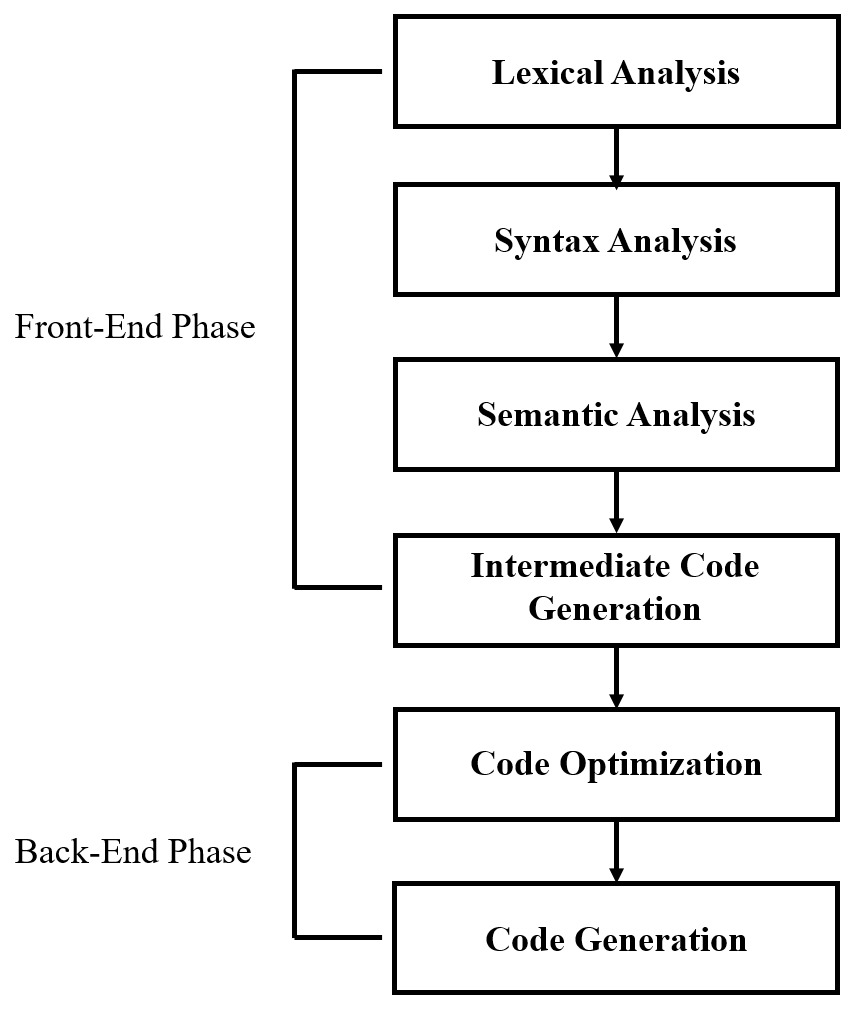
\includegraphics[scale=0.25]{basics_of_compiler/comp_stages.jpeg}
    \caption{Compiler Stages}
    \label{fig:comp_stages}
\end{figure}


\section{Front-End}
%TODO mention parsing here in a paragraph

\subsection{Lexical Analysis}
The compiler breaks down the source code into smaller units called lexemes, which are pieces of code that correspond to specific patterns in the code. These lexemes are then converted into tokens that can be used for syntax and semantic analyses.

\subsection{Syntax Analysis}
The compiler checks that the code follows the proper syntax for the programming language it is written in. This process is also called parsing. As part of this step, the compiler often creates abstract syntax trees in order to represent the logical structure of different parts of the code.

\subsection{Semantic Analysis}
The compiler checks that the code makes logical sense, going beyond syntax analysis by ensuring that the code is correct. For example, the compiler might check that variables have been declared correctly and given the appropriate data types. This process is known as semantic analysis.

\subsection{IR Code Generation}
After the source code has been analyzed for lexemes, syntax, and semantics, the compiler creates an intermediate representation (IR) of the code.
This intermediate code is going to be converted to machine code in the last two phases. These two phases are platform-dependent, meaning they are specific to a particular hardware architecture but the previous phases were not. Therefore, to create a new compiler, it is not necessary to start from scratch. Instead, it is possible to use the intermediate code from an existing compiler and build the final stages of the process for a specific platform. Because of that, we are interested in the back-end part for our project.

\section{Middle-End}

\subsection{Optimization}
The intermediate code is prepared for the final code generation step. This process does not change the meaning or functionality of the code, but it can make the program run faster and more efficiently.
A directed acyclic graph (DAG) used in the compiler design process might represent the dependencies between different instructions in the IR code, such as the order in which those instructions need to be executed or the data dependencies between them. The DAG can be used by the compiler to identify opportunities for optimization, such as removing unnecessary instructions, combining some of them, or rearranging the order of execution to reduce the number of resources required by the code.
%TODO we should mention SSA form as well

\section{Back-End}



\subsection{Target Code Generation}
The target code generator is the final stage of the compilation process, and its main function is to convert the optimized code into a form that the machine can understand. The optimized code is turned into a relocatable machine code. The relocatable machine code is the input to the linker and loader, which are responsible for combining the code with other necessary resources and preparing it for execution %\cite{tutorialcomp}. 
Target code generation can be divided into different parts:

\subsection{Instruction Selection} 
IR is the input of the code generation step, and it maps the IR into the target machine’s instruction set. There may be multiple ways for converting one representation, so the code generator tries to select the most suitable instructions.

\subsection{Register Allocation}
There may be many different variables/values in a program. The code generator decides which registers to use to keep these values.

\subsection{Instruction Scheduling}
The code generator determines the sequence in which instructions will be executed and creates schedules for the execution of those instructions.

